\documentclass[12pt]{standalone}
\usepackage[utf8]{inputenc}
\usepackage[T1]{fontenc}
\usepackage{times}
\usepackage{amsmath,amssymb}
\usepackage[dvipsnames,svgnames]{xcolor}
\usepackage{tikz}
\usetikzlibrary{calc, positioning, arrows.meta, decorations.pathreplacing}
\definecolor{dmrsfill}{HTML}{CDE2FB}
\definecolor{winblue}{HTML}{0D366B}
\definecolor{inksec}{HTML}{52514E}
% Adaptado de Bjornson et al. (2017), Fig. 2.1, p. 67: sem a divisao UL/DL (TDD);
% bloco = 1 PRB (12 subportadoras) durante T_c.
\begin{document}
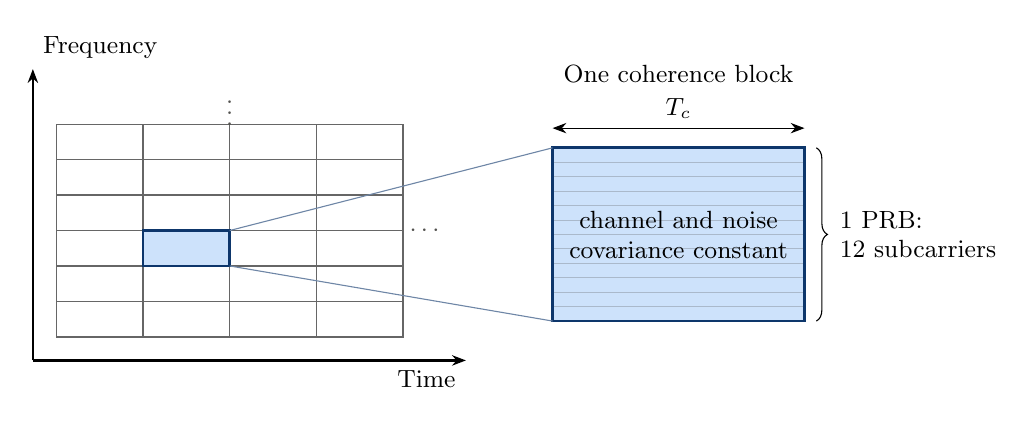
\begin{tikzpicture}[font=\fontsize{9}{10.8}\selectfont, >={Stealth[length=5pt]}]
\def\bw{1.1}  % largura de um bloco (T_c)
\def\bh{0.45} % altura de um bloco (1 PRB)
% eixos
\draw[->, line width=0.8pt] (-0.3,-0.3) -- (5.2,-0.3) node[below left] {Time};
\draw[->, line width=0.8pt] (-0.3,-0.3) -- (-0.3,3.4) node[above right] {Frequency};
% grade de blocos
\foreach \i in {0,...,3} \foreach \j in {0,...,5}
  \draw[black!60, line width=0.5pt] (\i*\bw,\j*\bh) rectangle ++(\bw,\bh);
\fill[dmrsfill] (1*\bw,2*\bh) rectangle ++(\bw,\bh);
\draw[winblue, line width=1pt] (1*\bw,2*\bh) rectangle ++(\bw,\bh);
\node[inksec] at (4*\bw+0.3,3*\bh) {$\cdots$};
\node[inksec] at (2*\bw,6*\bh+0.25) {$\vdots$};
% ampliacao de um bloco
\def\zx{6.3}\def\zy{0.2}\def\zw{3.2}\def\zh{2.2}
\fill[dmrsfill] (\zx,\zy) rectangle ++(\zw,\zh);
\foreach \k in {1,...,11} \draw[winblue!35, line width=0.3pt] (\zx,\zy+\k*\zh/12) -- ++(\zw,0);
\draw[winblue, line width=1pt] (\zx,\zy) rectangle ++(\zw,\zh);
\draw[winblue!60, line width=0.4pt] (2*\bw,3*\bh) -- (\zx,\zy+\zh);
\draw[winblue!60, line width=0.4pt] (2*\bw,2*\bh) -- (\zx,\zy);
\node[align=center] at (\zx+\zw/2,\zy+\zh/2) {channel and noise\\covariance constant};
\draw[<->] (\zx,\zy+\zh+0.25) -- node[above] {$T_c$} ++(\zw,0);
\draw[decorate, decoration={brace, amplitude=4pt}] (\zx+\zw+0.15,\zy+\zh) -- (\zx+\zw+0.15,\zy)
  node[midway, right=5pt, align=left] {1 PRB:\\12 subcarriers};
\node[above, align=center] at (\zx+\zw/2,\zy+\zh+0.7) {One coherence block};
\end{tikzpicture}
\end{document}
